\begin{enumerate}[label=\thechapter.\arabic*,ref=\thechapter.\theenumi]
\item A sinusoidal message signal having root mean square value of 4V and frequency of 1 kHz fed to a phase modulator with phase deviation constant 2 rad/volt. If the carrier signal is $c\brak{t} = 2\cos \brak{2\pi 10^6 t}$, the maximum instantaneous frequency of the phase modulated signal (rounded off to one decimal place) is \rule{1cm}{0.05mm} Hz. \hfill(GATE 2021 EC)\\
\solution\\
\iffalse
\let\negmedspace\undefined
\let\negthickspace\undefined
\documentclass[journal,12pt,twocolumn]{IEEEtran}
\usepackage{cite}
\usepackage{amsmath,amssymb,amsfonts,amsthm}
\usepackage{algorithmic}
\usepackage{graphicx}
\usepackage{textcomp}
\usepackage{xcolor}
\usepackage{txfonts}
\usepackage{listings}
\usepackage{enumitem}
\usepackage{mathtools}
\usepackage{gensymb}
\usepackage{comment}
\usepackage[breaklinks=true]{hyperref}
\usepackage{tkz-euclide} 
\usepackage{listings}
\usepackage{gvv}                                        
\def\inputGnumericTable{}                                 
\usepackage[latin1]{inputenc}                                
\usepackage{color}                                            
\usepackage{array}                                            
\usepackage{longtable}                                       
\usepackage{calc}                                             
\usepackage{multirow}                                         
\usepackage{hhline}                                           
\usepackage{ifthen}                                           
\usepackage{lscape}
\usepackage[center]{caption} % center the captions to figure

\newtheorem{theorem}{Theorem}[section]
\newtheorem{problem}{Problem}
\newtheorem{proposition}{Proposition}[section]
\newtheorem{lemma}{Lemma}[section]
\newtheorem{corollary}[theorem]{Corollary}
\newtheorem{example}{Example}[section]
\newtheorem{definition}[problem]{Definition}
\newcommand{\BEQA}{\begin{eqnarray}}
\newcommand{\EEQA}{\end{eqnarray}}
\newcommand{\define}{\stackrel{\triangle}{=}}
\theoremstyle{remark}
\newtheorem{rem}{Remark}
\begin{document}

\newcolumntype{M}[1]{>{\centering\arraybackslash}m{#1}}
\newcolumntype{N}{@{}m{0pt}@{}}

\bibliographystyle{IEEEtran}
\vspace{3cm}

\title{GATE 2021 ME 3Q} 
\author{ee23btech11223 - Soham Prabhakar More% <-this % stops a space
}
\maketitle
\newpage
\bigskip

\renewcommand{\thefigure}{\theenumi}
\renewcommand{\thetable}{\theenumi}

\bibliographystyle{IEEEtran}

\textbf{Question:} The Dirac-delta function $\brak{\delta\brak{t - t_0}}$ for $t, t_0 \in \Re$, has the following property
\begin{align}
    \int_{a}^{b}\phi\brak{t}\delta\brak{t - t_0}dt = 
    \begin{cases}
        \phi\brak{t_0}\quad a < t_0 < b\\
        0 \quad\quad otherwise
    \end{cases} \label{eq:2022.ME.3.1}
\end{align}

The Laplace Transform of the Dirac-delta function $\delta\brak{t - a}$ for $a > 0; \mathcal{L}\brak{\delta\brak{t - a}} = F\brak{s}$ is

\hfill{(GATE 2021 ME 3Q)}

\solution
\fi
\begin{table}[ht]
    \renewcommand\thetable{1}
\begin{tabular}{|c|c|}
    \hline 
    \textbf{Parameter}&\textbf{Description} \\
    \hline
    $F\brak{s}$ & Laplace transform of $\delta\brak{t - a}$ \\
    \hline
    $G\brak{f}$ & Fourier transform of $\delta\brak{t - a}$ \\
    \hline
    $H\brak{t}$ & Fourier transform of a function with period $T$ \\
    \hline
    $w_T\brak{t}$ & Delta Comb, $\sum_{k = -\infty}^{\infty}\delta\brak{t - kT}$ \\
    \hline
    $W_T\brak{t}$ & Fourier transform of $w_T\brak{t}$ \\
    \hline
\end{tabular}

\caption{Table of parameters}
\label{Table:2022.ME.3.1}


\end{table} \\

By \eqref{eq:2022.ME.3.1} and $a > 0$,
\begin{align}
    F\brak{s} &= \int_{0}^{\infty}\delta\brak{t - a}e^{-st}dt \\
    \therefore F\brak{s} &= e^{-as}
\end{align}

The fourier transform,
\begin{align}
    G\brak{f} &= \int_{-\infty}^{\infty}\delta\brak{t - a}e^{-2\pi jft}dt \\
    \therefore G\brak{f} &= e^{-j2\pi fa}
\end{align}
For a periodic signal the fourier transform is defined as:
\begin{align}
    H\brak{f} &= \sum_{k = -\infty}^{\infty}c_k\delta\brak{f - \frac{k}{T}}
\end{align}
where $c_k$ are the fourier series coefficients and $T$ is the period. Thus,
\begin{align}
    W_T\brak{f} &= \sum_{k = -\infty}^{\infty}c_k\delta\brak{f - \frac{k}{T}} \\
    c_k &= \frac{1}{T}\int_{-\frac{T}{2}}^{\frac{T}{2}}w_T\brak{t}e^{-j2\pi \frac{k}{T}f}dt \\
    c_k &= \frac{1}{T}\int_{-\frac{T}{2}}^{\frac{T}{2}}\brak{\sum_{k = -\infty}^{\infty}\delta\brak{t - kT}}e^{-j2\pi \frac{k}{T}f}dt \\
\end{align}
\begin{align}
    c_k &= \frac{1}{T}\sum_{k = -\infty}^{\infty}\int_{-\frac{T}{2}}^{\frac{T}{2}}\delta\brak{t - kT}e^{-j2\pi \frac{k}{T}f}dt \\
    c_k &= \frac{1}{T} \\
    W_T\brak{f} &= \frac{1}{T}\sum_{k = -\infty}^{\infty}\delta\brak{f - \frac{k}{T}} \\
    \therefore W_T\brak{f} &= \frac{1}{T}w_{\frac{1}{T}}\brak{f}
\end{align}
Thus, the fourier transform of impulse train is another impulse train.
%\begin{align}
%    f\brak{t} &\system{F} H\brak{f} \\
%    f\brak{t + T} &\system{F} e^{j2\pi fT}H\brak{f} \\
%    \because e^{j2\pi fT}H\brak{f} &= H\brak{f} \\
%    H\brak{f}\brak{1 - e^{j2\pi fT}} &= 0
%\end{align}
%Thus, $H\brak{f}$ is zero everywhere except at $f = \frac{n}{T}, n \in Z$
%\begin{align}
%    \therefore H\brak{f} &= \sum_{k = -\infty}^{\infty}c_k\delta\brak{f - \frac{k}{T}} \\
%    \because \sum_{k = -\infty}^{\infty}c_ke^{-j2\pi f\frac{k}{T}} &\system{F} H\brak{f}
%\end{align}
%$c_k$ are the fourier series coefficents of $h\brak{t}$,
%\begin{align}
%    c_k = \int_{-\frac{T}{2}}^{\frac{T}{2}}
%\end{align}
%\end{document}

\pagebreak
\item Two discrete-time linear time-invarient systems with impulse responses $h_1[n]=\delta[n-1]+\delta[n+1]$ and $h_2[n]=\delta[n]+\delta[n-1]$ are connected in cascade, where $\delta[n]$ is the Kronecker delta. The impulse response of the cascaded system is   \\
\begin{enumerate}[label=(\alph*)]
    \item $\delta[n-2]+\delta[n+1]$
    \item $\delta[n-1]\delta[n]+\delta[n+1]\delta[n-1]$
    \item $\delta[n-2]+\delta[n-1]+\delta[n]+\delta[n+1]$
    \item $\delta[n]\delta[n-1]+\delta[n-2]\delta[n+1]$
\end{enumerate} \hfill(GATE 2021 EE)\\
\solution
\input{2021/EE/7/gate7.tex}
\pagebreak
\item Consider a superheterodyne receiver tuned to 600 kHz. If the local oscillator feeds a 1000 kHz signal to the mixer, the image frequency (in integer) is \underline{\hspace{1cm}} kHz.
\hfill(GATE EC 2021)\\
\solution
\input{2021/EC/50/50.tex}
\pagebreak
\item Consider a unity feedback system with closed loop transfer function
\begin{align*}
\frac{C\brak{s}}{R\brak{s}} &= \frac{s + 90}{s^2 + 10s + 90}
\end{align*}
The steady state error with respect to a unit ramp input is \rule{1cm}{0.15mm} .
\hfill(GATE 2021 BM) \\
\solution
\iffalse
\let\negmedspace\undefined
\let\negthickspace\undefined
\documentclass[journal,12pt,twocolumn]{IEEEtran}
\usepackage{cite}
\usepackage{amsmath,amssymb,amsfonts,amsthm}
\usepackage{algorithmic}
\usepackage{graphicx}
\usepackage{textcomp}
\usepackage{xcolor}
\usepackage{txfonts}
\usepackage{listings}
\usepackage{enumitem}
\usepackage{mathtools}
\usepackage{gensymb}
\usepackage{comment}
\usepackage[breaklinks=true]{hyperref}
\usepackage{tkz-euclide} 
\usepackage{listings}
\usepackage{gvv}                                        
\def\inputGnumericTable{}                                 
\usepackage[latin1]{inputenc}                                
\usepackage{color}                                            
\usepackage{array}                                            
\usepackage{longtable}                                       
\usepackage{calc}                                             
\usepackage{multirow}                                         
\usepackage{hhline}                                           
\usepackage{ifthen}                                           
\usepackage{lscape}
\usepackage[center]{caption} % center the captions to figure

\newtheorem{theorem}{Theorem}[section]
\newtheorem{problem}{Problem}
\newtheorem{proposition}{Proposition}[section]
\newtheorem{lemma}{Lemma}[section]
\newtheorem{corollary}[theorem]{Corollary}
\newtheorem{example}{Example}[section]
\newtheorem{definition}[problem]{Definition}
\newcommand{\BEQA}{\begin{eqnarray}}
\newcommand{\EEQA}{\end{eqnarray}}
\newcommand{\define}{\stackrel{\triangle}{=}}
\theoremstyle{remark}
\newtheorem{rem}{Remark}
\begin{document}

\newcolumntype{M}[1]{>{\centering\arraybackslash}m{#1}}
\newcolumntype{N}{@{}m{0pt}@{}}

\bibliographystyle{IEEEtran}
\vspace{3cm}

\title{GATE 2021 ME 3Q} 
\author{ee23btech11223 - Soham Prabhakar More% <-this % stops a space
}
\maketitle
\newpage
\bigskip

\renewcommand{\thefigure}{\theenumi}
\renewcommand{\thetable}{\theenumi}

\bibliographystyle{IEEEtran}

\textbf{Question:} The Dirac-delta function $\brak{\delta\brak{t - t_0}}$ for $t, t_0 \in \Re$, has the following property
\begin{align}
    \int_{a}^{b}\phi\brak{t}\delta\brak{t - t_0}dt = 
    \begin{cases}
        \phi\brak{t_0}\quad a < t_0 < b\\
        0 \quad\quad otherwise
    \end{cases} \label{eq:2022.ME.3.1}
\end{align}

The Laplace Transform of the Dirac-delta function $\delta\brak{t - a}$ for $a > 0; \mathcal{L}\brak{\delta\brak{t - a}} = F\brak{s}$ is

\hfill{(GATE 2021 ME 3Q)}

\solution
\fi
\begin{table}[ht]
    \renewcommand\thetable{1}
\begin{tabular}{|c|c|}
    \hline 
    \textbf{Parameter}&\textbf{Description} \\
    \hline
    $F\brak{s}$ & Laplace transform of $\delta\brak{t - a}$ \\
    \hline
    $G\brak{f}$ & Fourier transform of $\delta\brak{t - a}$ \\
    \hline
    $H\brak{t}$ & Fourier transform of a function with period $T$ \\
    \hline
    $w_T\brak{t}$ & Delta Comb, $\sum_{k = -\infty}^{\infty}\delta\brak{t - kT}$ \\
    \hline
    $W_T\brak{t}$ & Fourier transform of $w_T\brak{t}$ \\
    \hline
\end{tabular}

\caption{Table of parameters}
\label{Table:2022.ME.3.1}


\end{table} \\

By \eqref{eq:2022.ME.3.1} and $a > 0$,
\begin{align}
    F\brak{s} &= \int_{0}^{\infty}\delta\brak{t - a}e^{-st}dt \\
    \therefore F\brak{s} &= e^{-as}
\end{align}

The fourier transform,
\begin{align}
    G\brak{f} &= \int_{-\infty}^{\infty}\delta\brak{t - a}e^{-2\pi jft}dt \\
    \therefore G\brak{f} &= e^{-j2\pi fa}
\end{align}
For a periodic signal the fourier transform is defined as:
\begin{align}
    H\brak{f} &= \sum_{k = -\infty}^{\infty}c_k\delta\brak{f - \frac{k}{T}}
\end{align}
where $c_k$ are the fourier series coefficients and $T$ is the period. Thus,
\begin{align}
    W_T\brak{f} &= \sum_{k = -\infty}^{\infty}c_k\delta\brak{f - \frac{k}{T}} \\
    c_k &= \frac{1}{T}\int_{-\frac{T}{2}}^{\frac{T}{2}}w_T\brak{t}e^{-j2\pi \frac{k}{T}f}dt \\
    c_k &= \frac{1}{T}\int_{-\frac{T}{2}}^{\frac{T}{2}}\brak{\sum_{k = -\infty}^{\infty}\delta\brak{t - kT}}e^{-j2\pi \frac{k}{T}f}dt \\
\end{align}
\begin{align}
    c_k &= \frac{1}{T}\sum_{k = -\infty}^{\infty}\int_{-\frac{T}{2}}^{\frac{T}{2}}\delta\brak{t - kT}e^{-j2\pi \frac{k}{T}f}dt \\
    c_k &= \frac{1}{T} \\
    W_T\brak{f} &= \frac{1}{T}\sum_{k = -\infty}^{\infty}\delta\brak{f - \frac{k}{T}} \\
    \therefore W_T\brak{f} &= \frac{1}{T}w_{\frac{1}{T}}\brak{f}
\end{align}
Thus, the fourier transform of impulse train is another impulse train.
%\begin{align}
%    f\brak{t} &\system{F} H\brak{f} \\
%    f\brak{t + T} &\system{F} e^{j2\pi fT}H\brak{f} \\
%    \because e^{j2\pi fT}H\brak{f} &= H\brak{f} \\
%    H\brak{f}\brak{1 - e^{j2\pi fT}} &= 0
%\end{align}
%Thus, $H\brak{f}$ is zero everywhere except at $f = \frac{n}{T}, n \in Z$
%\begin{align}
%    \therefore H\brak{f} &= \sum_{k = -\infty}^{\infty}c_k\delta\brak{f - \frac{k}{T}} \\
%    \because \sum_{k = -\infty}^{\infty}c_ke^{-j2\pi f\frac{k}{T}} &\system{F} H\brak{f}
%\end{align}
%$c_k$ are the fourier series coefficents of $h\brak{t}$,
%\begin{align}
%    c_k = \int_{-\frac{T}{2}}^{\frac{T}{2}}
%\end{align}
%\end{document}

\item A unit step input is applied to a system with impulse response H\brak{s} = $\frac{1- \frac{s}{\omega{_z}}}{1+\frac{s}{\omega{_p}}}$ at t=0. The output of the system $y\brak{t}$ at t=$0^+$ is:
\begin{enumerate}[label=\alph*)]
 \item 1
 \item $-\frac{\omega{_z}}{\omega{_p}}$
 \item $-\frac{\omega{_p}}{\omega{_z}}$
 \item 0
\end{enumerate} \hfill(GATE 2021 BM)\\
\solution
\input{2021/BM/27/27.tex}

\item In the block diagram shown below, an infinite tap FIR filter with transfer function $H\brak{z}=\frac{Y\brak{z}}{X\brak{z}}$ is realized. If $H\brak{z}=\frac{1}{1-0.5z^{-1}}$.\\the value of $\alpha$ is
\begin{figure}[h]
    \includegraphics[width=1\columnwidth]{2021/BM/31/figs/questionfig.png}
    \label{fig:question31bm}
\end{figure} \hfill(GATE 2021 BM)\\
\solution
\input{2021/BM/31/Assignmentbm31.tex}
\pagebreak
\item A unity feedback system that uses proportional-integral (PI) control is shown in the figure.
 \begin{figure}[!ht]    
    \centering
\graphicspath{ {2021/EC/48/figs} }
\includegraphics[width=\columnwidth]{figure_1}
\label{figure:ee25-gate4-graph}
\end{figure}
The stability of the overall system is controlled by tuning the PI control parameters $K_p$ and $K_i$. The maximum value of $K_i$ that can be chosen so as to keep the overall system stable or, in the worst case, marginally stable (\textit{rounded off to three decimal places}) is?
\hfill{(GATE EC 2021)}\\
\solution
\input{2021/EC/48/ec-48.tex}
\pagebreak
\item In the given figure, plant $G_p(s)=\frac{2.2}{(1+0.1s)(1+0.4s)(1+1.2s)}$ and compensator $G_c(s)=K\brak{\frac{1+T_1s}{1+T_2s}}$ . The external disturbance input is D(s). It is desired that when the disturbance is a unit step, the steady-state error should not exceed 0.1 unit. The minimum value of K is 
\hfill{(GATE EE 2021)}\\
\begin{figure}[h!]
    \centering
    \includegraphics[width=\columnwidth]{2021/EE/47/figs/fig.png}
    \caption{}
    \label{fig:sr40}
\end{figure}
\\
\solution
\input{2021/EE/47/gate.tex}
\pagebreak
\item For the closed loop system shown , the transfer function $\frac{E(s)}{R(s)}$ is \\
\begin{figure}[ht]
	\centering
	\includegraphics[width=1\linewidth]{2021/EE/11/figs/questiondia.png}
\end{figure}
\begin{enumerate}[label = (\alph*)]
	\item $\frac{G}{1+GH}$
	\item $\frac{GH}{1+GH}$
	\item $\frac{1}{1+GH}$
	\item $\frac{1}{1+G}$
\end{enumerate} \hfill{(GATE EE 2021)}\\
\iffalse
\let\negmedspace\undefined
\let\negthickspace\undefined
\documentclass[journal,12pt,twocolumn]{IEEEtran}
\usepackage{cite}
\usepackage{amsmath,amssymb,amsfonts,amsthm}
\usepackage{algorithmic}
\usepackage{graphicx}
\usepackage{textcomp}
\usepackage{xcolor}
\usepackage{txfonts}
\usepackage{listings}
\usepackage{enumitem}
\usepackage{mathtools}
\usepackage{gensymb}
\usepackage{comment}
\usepackage[breaklinks=true]{hyperref}
\usepackage{tkz-euclide} 
\usepackage{listings}
\usepackage{gvv}                                        
\def\inputGnumericTable{}                                 
\usepackage[latin1]{inputenc}                                
\usepackage{color}                                            
\usepackage{array}                                            
\usepackage{longtable}                                       
\usepackage{calc}                                             
\usepackage{multirow}                                         
\usepackage{hhline}                                           
\usepackage{ifthen}                                           
\usepackage{lscape}
\usepackage[center]{caption} % center the captions to figure

\newtheorem{theorem}{Theorem}[section]
\newtheorem{problem}{Problem}
\newtheorem{proposition}{Proposition}[section]
\newtheorem{lemma}{Lemma}[section]
\newtheorem{corollary}[theorem]{Corollary}
\newtheorem{example}{Example}[section]
\newtheorem{definition}[problem]{Definition}
\newcommand{\BEQA}{\begin{eqnarray}}
\newcommand{\EEQA}{\end{eqnarray}}
\newcommand{\define}{\stackrel{\triangle}{=}}
\theoremstyle{remark}
\newtheorem{rem}{Remark}
\begin{document}

\newcolumntype{M}[1]{>{\centering\arraybackslash}m{#1}}
\newcolumntype{N}{@{}m{0pt}@{}}

\bibliographystyle{IEEEtran}
\vspace{3cm}

\title{GATE 2021 ME 3Q} 
\author{ee23btech11223 - Soham Prabhakar More% <-this % stops a space
}
\maketitle
\newpage
\bigskip

\renewcommand{\thefigure}{\theenumi}
\renewcommand{\thetable}{\theenumi}

\bibliographystyle{IEEEtran}

\textbf{Question:} The Dirac-delta function $\brak{\delta\brak{t - t_0}}$ for $t, t_0 \in \Re$, has the following property
\begin{align}
    \int_{a}^{b}\phi\brak{t}\delta\brak{t - t_0}dt = 
    \begin{cases}
        \phi\brak{t_0}\quad a < t_0 < b\\
        0 \quad\quad otherwise
    \end{cases} \label{eq:2022.ME.3.1}
\end{align}

The Laplace Transform of the Dirac-delta function $\delta\brak{t - a}$ for $a > 0; \mathcal{L}\brak{\delta\brak{t - a}} = F\brak{s}$ is

\hfill{(GATE 2021 ME 3Q)}

\solution
\fi
\begin{table}[ht]
    \renewcommand\thetable{1}
\begin{tabular}{|c|c|}
    \hline 
    \textbf{Parameter}&\textbf{Description} \\
    \hline
    $F\brak{s}$ & Laplace transform of $\delta\brak{t - a}$ \\
    \hline
    $G\brak{f}$ & Fourier transform of $\delta\brak{t - a}$ \\
    \hline
    $H\brak{t}$ & Fourier transform of a function with period $T$ \\
    \hline
    $w_T\brak{t}$ & Delta Comb, $\sum_{k = -\infty}^{\infty}\delta\brak{t - kT}$ \\
    \hline
    $W_T\brak{t}$ & Fourier transform of $w_T\brak{t}$ \\
    \hline
\end{tabular}

\caption{Table of parameters}
\label{Table:2022.ME.3.1}


\end{table} \\

By \eqref{eq:2022.ME.3.1} and $a > 0$,
\begin{align}
    F\brak{s} &= \int_{0}^{\infty}\delta\brak{t - a}e^{-st}dt \\
    \therefore F\brak{s} &= e^{-as}
\end{align}

The fourier transform,
\begin{align}
    G\brak{f} &= \int_{-\infty}^{\infty}\delta\brak{t - a}e^{-2\pi jft}dt \\
    \therefore G\brak{f} &= e^{-j2\pi fa}
\end{align}
For a periodic signal the fourier transform is defined as:
\begin{align}
    H\brak{f} &= \sum_{k = -\infty}^{\infty}c_k\delta\brak{f - \frac{k}{T}}
\end{align}
where $c_k$ are the fourier series coefficients and $T$ is the period. Thus,
\begin{align}
    W_T\brak{f} &= \sum_{k = -\infty}^{\infty}c_k\delta\brak{f - \frac{k}{T}} \\
    c_k &= \frac{1}{T}\int_{-\frac{T}{2}}^{\frac{T}{2}}w_T\brak{t}e^{-j2\pi \frac{k}{T}f}dt \\
    c_k &= \frac{1}{T}\int_{-\frac{T}{2}}^{\frac{T}{2}}\brak{\sum_{k = -\infty}^{\infty}\delta\brak{t - kT}}e^{-j2\pi \frac{k}{T}f}dt \\
\end{align}
\begin{align}
    c_k &= \frac{1}{T}\sum_{k = -\infty}^{\infty}\int_{-\frac{T}{2}}^{\frac{T}{2}}\delta\brak{t - kT}e^{-j2\pi \frac{k}{T}f}dt \\
    c_k &= \frac{1}{T} \\
    W_T\brak{f} &= \frac{1}{T}\sum_{k = -\infty}^{\infty}\delta\brak{f - \frac{k}{T}} \\
    \therefore W_T\brak{f} &= \frac{1}{T}w_{\frac{1}{T}}\brak{f}
\end{align}
Thus, the fourier transform of impulse train is another impulse train.
%\begin{align}
%    f\brak{t} &\system{F} H\brak{f} \\
%    f\brak{t + T} &\system{F} e^{j2\pi fT}H\brak{f} \\
%    \because e^{j2\pi fT}H\brak{f} &= H\brak{f} \\
%    H\brak{f}\brak{1 - e^{j2\pi fT}} &= 0
%\end{align}
%Thus, $H\brak{f}$ is zero everywhere except at $f = \frac{n}{T}, n \in Z$
%\begin{align}
%    \therefore H\brak{f} &= \sum_{k = -\infty}^{\infty}c_k\delta\brak{f - \frac{k}{T}} \\
%    \because \sum_{k = -\infty}^{\infty}c_ke^{-j2\pi f\frac{k}{T}} &\system{F} H\brak{f}
%\end{align}
%$c_k$ are the fourier series coefficents of $h\brak{t}$,
%\begin{align}
%    c_k = \int_{-\frac{T}{2}}^{\frac{T}{2}}
%\end{align}
%\end{document}

\pagebreak

Consider two 16-point sequences x\sbrak{n} and h\sbrak{n}. Let the linear convolution of x\sbrak{n} and h\sbrak{n} be denoted by y\sbrak{n}, while z\sbrak{n} denotes the 16-point inverse discrete Fourier transform \brak{IDFT} of the product of the 16-point DFTs of x\brak{n} and h\sbrak{n}. The values of k for which z\sbrak{k} = y\sbrak{k} are 
\begin{enumerate}
    \item $k = 0, 1, 2, 3, ... , 15$
    \item $k = 0$
    \item $k = 15$
    \item $k = 0$ and $k = 15$
\end{enumerate}
\hfill(GATE EC 2021)\\
\solution
\input{2021/EC/5/ec5.tex}
\pagebreak
\item The input signal shown below \\
\input{2021/IN/44/figs/xn}\\
is passed through the filter with following taps\\
\input{2021/IN/44/figs/n}\\
The number of non-zero output samples is \underline{\hspace{1cm}}.\\
\hfill(GATE IN 2021)
\solution
\iffalse
\let\negmedspace\undefined
\let\negthickspace\undefined
\documentclass[journal,12pt,twocolumn]{IEEEtran}
\usepackage{cite}
\usepackage{amsmath,amssymb,amsfonts,amsthm}
\usepackage{algorithmic}
\usepackage{graphicx}
\usepackage{textcomp}
\usepackage{xcolor}
\usepackage{txfonts}
\usepackage{listings}
\usepackage{enumitem}
\usepackage{mathtools}
\usepackage{gensymb}
\usepackage{comment}
\usepackage[breaklinks=true]{hyperref}
\usepackage{tkz-euclide} 
\usepackage{listings}
\usepackage{gvv}                                        
\def\inputGnumericTable{}                                 
\usepackage[latin1]{inputenc}                                
\usepackage{color}                                            
\usepackage{array}                                            
\usepackage{longtable}                                       
\usepackage{calc}                                             
\usepackage{multirow}                                         
\usepackage{hhline}                                           
\usepackage{ifthen}                                           
\usepackage{lscape}
\usepackage[center]{caption} % center the captions to figure

\newtheorem{theorem}{Theorem}[section]
\newtheorem{problem}{Problem}
\newtheorem{proposition}{Proposition}[section]
\newtheorem{lemma}{Lemma}[section]
\newtheorem{corollary}[theorem]{Corollary}
\newtheorem{example}{Example}[section]
\newtheorem{definition}[problem]{Definition}
\newcommand{\BEQA}{\begin{eqnarray}}
\newcommand{\EEQA}{\end{eqnarray}}
\newcommand{\define}{\stackrel{\triangle}{=}}
\theoremstyle{remark}
\newtheorem{rem}{Remark}
\begin{document}

\newcolumntype{M}[1]{>{\centering\arraybackslash}m{#1}}
\newcolumntype{N}{@{}m{0pt}@{}}

\bibliographystyle{IEEEtran}
\vspace{3cm}

\title{GATE 2021 ME 3Q} 
\author{ee23btech11223 - Soham Prabhakar More% <-this % stops a space
}
\maketitle
\newpage
\bigskip

\renewcommand{\thefigure}{\theenumi}
\renewcommand{\thetable}{\theenumi}

\bibliographystyle{IEEEtran}

\textbf{Question:} The Dirac-delta function $\brak{\delta\brak{t - t_0}}$ for $t, t_0 \in \Re$, has the following property
\begin{align}
    \int_{a}^{b}\phi\brak{t}\delta\brak{t - t_0}dt = 
    \begin{cases}
        \phi\brak{t_0}\quad a < t_0 < b\\
        0 \quad\quad otherwise
    \end{cases} \label{eq:2022.ME.3.1}
\end{align}

The Laplace Transform of the Dirac-delta function $\delta\brak{t - a}$ for $a > 0; \mathcal{L}\brak{\delta\brak{t - a}} = F\brak{s}$ is

\hfill{(GATE 2021 ME 3Q)}

\solution
\fi
\begin{table}[ht]
    \renewcommand\thetable{1}
\begin{tabular}{|c|c|}
    \hline 
    \textbf{Parameter}&\textbf{Description} \\
    \hline
    $F\brak{s}$ & Laplace transform of $\delta\brak{t - a}$ \\
    \hline
    $G\brak{f}$ & Fourier transform of $\delta\brak{t - a}$ \\
    \hline
    $H\brak{t}$ & Fourier transform of a function with period $T$ \\
    \hline
    $w_T\brak{t}$ & Delta Comb, $\sum_{k = -\infty}^{\infty}\delta\brak{t - kT}$ \\
    \hline
    $W_T\brak{t}$ & Fourier transform of $w_T\brak{t}$ \\
    \hline
\end{tabular}

\caption{Table of parameters}
\label{Table:2022.ME.3.1}


\end{table} \\

By \eqref{eq:2022.ME.3.1} and $a > 0$,
\begin{align}
    F\brak{s} &= \int_{0}^{\infty}\delta\brak{t - a}e^{-st}dt \\
    \therefore F\brak{s} &= e^{-as}
\end{align}

The fourier transform,
\begin{align}
    G\brak{f} &= \int_{-\infty}^{\infty}\delta\brak{t - a}e^{-2\pi jft}dt \\
    \therefore G\brak{f} &= e^{-j2\pi fa}
\end{align}
For a periodic signal the fourier transform is defined as:
\begin{align}
    H\brak{f} &= \sum_{k = -\infty}^{\infty}c_k\delta\brak{f - \frac{k}{T}}
\end{align}
where $c_k$ are the fourier series coefficients and $T$ is the period. Thus,
\begin{align}
    W_T\brak{f} &= \sum_{k = -\infty}^{\infty}c_k\delta\brak{f - \frac{k}{T}} \\
    c_k &= \frac{1}{T}\int_{-\frac{T}{2}}^{\frac{T}{2}}w_T\brak{t}e^{-j2\pi \frac{k}{T}f}dt \\
    c_k &= \frac{1}{T}\int_{-\frac{T}{2}}^{\frac{T}{2}}\brak{\sum_{k = -\infty}^{\infty}\delta\brak{t - kT}}e^{-j2\pi \frac{k}{T}f}dt \\
\end{align}
\begin{align}
    c_k &= \frac{1}{T}\sum_{k = -\infty}^{\infty}\int_{-\frac{T}{2}}^{\frac{T}{2}}\delta\brak{t - kT}e^{-j2\pi \frac{k}{T}f}dt \\
    c_k &= \frac{1}{T} \\
    W_T\brak{f} &= \frac{1}{T}\sum_{k = -\infty}^{\infty}\delta\brak{f - \frac{k}{T}} \\
    \therefore W_T\brak{f} &= \frac{1}{T}w_{\frac{1}{T}}\brak{f}
\end{align}
Thus, the fourier transform of impulse train is another impulse train.
%\begin{align}
%    f\brak{t} &\system{F} H\brak{f} \\
%    f\brak{t + T} &\system{F} e^{j2\pi fT}H\brak{f} \\
%    \because e^{j2\pi fT}H\brak{f} &= H\brak{f} \\
%    H\brak{f}\brak{1 - e^{j2\pi fT}} &= 0
%\end{align}
%Thus, $H\brak{f}$ is zero everywhere except at $f = \frac{n}{T}, n \in Z$
%\begin{align}
%    \therefore H\brak{f} &= \sum_{k = -\infty}^{\infty}c_k\delta\brak{f - \frac{k}{T}} \\
%    \because \sum_{k = -\infty}^{\infty}c_ke^{-j2\pi f\frac{k}{T}} &\system{F} H\brak{f}
%\end{align}
%$c_k$ are the fourier series coefficents of $h\brak{t}$,
%\begin{align}
%    c_k = \int_{-\frac{T}{2}}^{\frac{T}{2}}
%\end{align}
%\end{document}

\pagebreak
\item A sinusoid $(\sqrt{2}sin(t))\mu(t)$,where $\mu(t)$ is the step input,is applied to a system with transfer function G(s)=$\frac{1}{1+s}$.The amplitude of the steady state output is\hfill{(GATE IN 2021)}\\
\solution
\input{2021/IN/45/gate21.in.45.tex}
\pagebreak
\item The block diagram of a feedback control system is shown in the figure .
\begin{center}
\includegraphics[width=0.5\textwidth]{2021/EC/13/figs/figure1.png}
\end{center}
The transfer function $\frac{Y(s)}{X(s)}$ of the system is :
\hfill(GATE 2021 EC)\\
\solution
\iffalse
\let\negmedspace\undefined
\let\negthickspace\undefined
\documentclass[journal,12pt,onecolumn]{IEEEtran}
\usepackage{cite}
\usepackage{amsmath,amssymb,amsfonts,amsthm}

\usepackage{graphicx}
\usepackage{textcomp}
\usepackage{xcolor}
\usepackage{txfonts}
\usepackage{listings}
\usepackage{enumitem}
\usepackage{mathtools}
\usepackage{gensymb}
\usepackage[breaklinks=true]{hyperref}
\usepackage{tkz-euclide} % loads  TikZ and tkz-base
\usepackage{listings}
\usepackage{gvv}
\usepackage{booktabs}

%
%\usepackage{setspace}
%\usepackage{gensymb}
%\doublespacing
%\singlespacing

%\usepackage{graphicx}
%\usepackage{amssymb}
%\usepackage{relsize}
%\usepackage[cmex10]{amsmath}
%\usepackage{amsthm}
%\interdisplaylinepenalty=2500
%\savesymbol{iint}
%\usepackage{txfonts}
%\restoresymbol{TXF}{iint}
%\usepackage{wasysym}
%\usepackage{amsthm}
%\usepackage{iithtlc}
%\usepackage{mathrsfs}
%\usepackage{txfonts}
%\usepackage{stfloats}
%\usepackage{bm}
%\usepackage{cite}
%\usepackage{cases}
%\usepackage{subfig}
%\usepackage{xtab}
%\usepackage{longtable}
%\usepackage{multirow}

%\usepackage{algpseudocode}
%\usepackage{enumitem}
%\usepackage{mathtools}
%\usepackage{tikz}
%\usepackage{circuitikz}
%\usepackage{verbatim}
%\usepackage{tfrupee}
%\usepackage{stmaryrd}
%\usetkzobj{all}
%    \usepackage{color}                                            %%
%    \usepackage{array}                                            %%
%    \usepackage{longtable}                                        %%
%    \usepackage{calc}                                             %%
%    \usepackage{multirow}                                         %%
%    \usepackage{hhline}                                           %%
%    \usepackage{ifthen}                                           %%
  %optionally (for landscape tables embedded in another document): %%
%    \usepackage{lscape}     
%\usepackage{multicol}
%\usepackage{chngcntr}
%\usepackage{enumerate}

%\usepackage{wasysym}
%\documentclass[conference]{IEEEtran}
%\IEEEoverridecommandlockouts
% The preceding line is only needed to identify funding in the first footnote. If that is unneeded, please comment it out.

\newtheorem{theorem}{Theorem}[section]
\newtheorem{problem}{Problem}
\newtheorem{proposition}{Proposition}[section]
\newtheorem{lemma}{Lemma}[section]
\newtheorem{corollary}[theorem]{Corollary}
\newtheorem{example}{Example}[section]
\newtheorem{definition}[problem]{Definition}
%\newtheorem{thm}{Theorem}[section] 
%\newtheorem{defn}[thm]{Definition}
%\newtheorem{algorithm}{Algorithm}[section]
%\newtheorem{cor}{Corollary}
\newcommand{\BEQA}{\begin{eqnarray}}
\newcommand{\EEQA}{\end{eqnarray}}
\newcommand{\define}{\stackrel{\triangle}{=}}
\theoremstyle{remark}
\newtheorem{rem}{Remark}

%\bibliographystyle{ieeetr}
\begin{document}
%

\bibliographystyle{IEEEtran}


\vspace{3cm}

\title{
%	\logo{
Gate 2021 Assignment 

\large{EE:1205 Signals and Systems}

Indian Institute of Technology, Hyderabad
%	}
}
\author{Abhey Garg

EE23BTECH11202
}	


% make the title area
\maketitle



%\tableofcontents


\renewcommand{\thefigure}{\theenumi}
\renewcommand{\thetable}{\theenumi}
%\renewcommand{\theequation}{\theenumi}

\section{Question EC 13}
The block diagram of a feedback control system is shown in the figure .
\begin{center}
\includegraphics[width=0.5\textwidth]{2021/EC/13/figs/figure1.png}
\end{center}
The transfer function $\frac{Y(s)}{X(s)}$ of the system is :
\hfill(GATE 2021 EC)
\section{Solution}
\fi
\begin{table}[ht]
\centering
\setlength{\extrarowheight}{8pt}
\caption{Input Parameters}
\begin{tabular}{|c|l|l|} 
\hline
\textbf{Parameter} & \textbf{Used to denote} & \textbf{Values} \\
\hline
$n$ & Number of forward paths & \multicolumn{1}{|p{1.3cm}|}{\centering $2$ }\\
\hline
$\Delta_k$ & The value of $\Delta$ which is not touching the $k^{th} $ forward path & \multicolumn{1}{|p{1.3cm}|}{\centering $\Delta_1 = 1 , \Delta_2 = 1$ } \\
\hline
$\Delta$ & 1 - sum of the loop gains & \multicolumn{1}{|p{1.3cm}|}{\centering $1-G_1H$ } \\
\hline
$P_k$ & $k^{th}$ forward path gain & \multicolumn{1}{|p{1.3cm}|}{\centering $P_1 = G_1 , P_2 = G_2$ } \\
\hline
\end{tabular}
 \vspace{4mm}
\end{table}

According to Mason's gain formula , transfer function can be given as :
\begin{align}
\text{TF } &= \frac{\sum_{k-1}^{n} P_k \Delta_k}{\Delta} = \frac{P_1\Delta_1 + P_2\Delta_2}{\Delta} \\
&= \frac{G_1 + G_2 }{1 + G_1 H}
\end{align}

\pagebreak
\item Consider a unity feedback configuration with a plant and a PID controller as shown in the figure. $G(s) = \frac{1}{(s+1)(s+3)} $ and $ C(s) = \frac{K(s+3+j)(s+3-j)}{s}$ with K being scalar . The closed loop is :
\begin{center}
\includegraphics[width=0.5\textwidth]{2021/IN/29/figs/figure1.jpg}
\end{center}
\begin{enumerate}
\item[A]only stable for $K < 0$
\item[B]stable for all value of K
\item[C]only stable for $K > 0$
\item[D]only stable for K between –1 and +1
\end{enumerate}
\hfill(GATE 2021 IN)\\
\solution
\iffalse
\let\negmedspace\undefined
\let\negthickspace\undefined
\documentclass[journal,12pt,onecolumn]{IEEEtran}
\usepackage{cite}
\usepackage{amsmath,amssymb,amsfonts,amsthm}

\usepackage{graphicx}
\usepackage{textcomp}
\usepackage{xcolor}
\usepackage{txfonts}
\usepackage{listings}
\usepackage{enumitem}
\usepackage{mathtools}
\usepackage{gensymb}
\usepackage[breaklinks=true]{hyperref}
\usepackage{tkz-euclide} % loads  TikZ and tkz-base
\usepackage{listings}
\usepackage{gvv}
\usepackage{booktabs}

%
%\usepackage{setspace}
%\usepackage{gensymb}
%\doublespacing
%\singlespacing

%\usepackage{graphicx}
%\usepackage{amssymb}
%\usepackage{relsize}
%\usepackage[cmex10]{amsmath}
%\usepackage{amsthm}
%\interdisplaylinepenalty=2500
%\savesymbol{iint}
%\usepackage{txfonts}
%\restoresymbol{TXF}{iint}
%\usepackage{wasysym}
%\usepackage{amsthm}
%\usepackage{iithtlc}
%\usepackage{mathrsfs}
%\usepackage{txfonts}
%\usepackage{stfloats}
%\usepackage{bm}
%\usepackage{cite}
%\usepackage{cases}
%\usepackage{subfig}
%\usepackage{xtab}
%\usepackage{longtable}
%\usepackage{multirow}

%\usepackage{algpseudocode}
%\usepackage{enumitem}
%\usepackage{mathtools}
%\usepackage{tikz}
%\usepackage{circuitikz}
%\usepackage{verbatim}
%\usepackage{tfrupee}
%\usepackage{stmaryrd}
%\usetkzobj{all}
%    \usepackage{color}                                            %%
%    \usepackage{array}                                            %%
%    \usepackage{longtable}                                        %%
%    \usepackage{calc}                                             %%
%    \usepackage{multirow}                                         %%
%    \usepackage{hhline}                                           %%
%    \usepackage{ifthen}                                           %%
  %optionally (for landscape tables embedded in another document): %%
%    \usepackage{lscape}     
%\usepackage{multicol}
%\usepackage{chngcntr}
%\usepackage{enumerate}

%\usepackage{wasysym}
%\documentclass[conference]{IEEEtran}
%\IEEEoverridecommandlockouts
% The preceding line is only needed to identify funding in the first footnote. If that is unneeded, please comment it out.

\newtheorem{theorem}{Theorem}[section]
\newtheorem{problem}{Problem}
\newtheorem{proposition}{Proposition}[section]
\newtheorem{lemma}{Lemma}[section]
\newtheorem{corollary}[theorem]{Corollary}
\newtheorem{example}{Example}[section]
\newtheorem{definition}[problem]{Definition}
%\newtheorem{thm}{Theorem}[section] 
%\newtheorem{defn}[thm]{Definition}
%\newtheorem{algorithm}{Algorithm}[section]
%\newtheorem{cor}{Corollary}
\newcommand{\BEQA}{\begin{eqnarray}}
\newcommand{\EEQA}{\end{eqnarray}}
\newcommand{\define}{\stackrel{\triangle}{=}}
\theoremstyle{remark}
\newtheorem{rem}{Remark}

%\bibliographystyle{ieeetr}
\begin{document}
%

\bibliographystyle{IEEEtran}


\vspace{3cm}

\title{
%	\logo{
Gate 2021 Assignment 

\large{EE:1205 Signals and Systems}

Indian Institute of Technology, Hyderabad
%	}
}
\author{Abhey Garg

EE23BTECH11202
}	


% make the title area
\maketitle



%\tableofcontents


\renewcommand{\thefigure}{\theenumi}
\renewcommand{\thetable}{\theenumi}
%\renewcommand{\theequation}{\theenumi}

\section{Question IN 02}
Consider a unity feedback configuration with a plant and a PID controller as shown in the figure. $G(s) = \frac{1}{(s+1)(s+3)} $ and $ C(s) = \frac{K(s+3+j)(s+3-j)}{s}$ with K being scalar . The closed loop is :
\begin{center}
\includegraphics[width=0.5\textwidth]{2021/IN/29/figs/figure1.jpg}
\end{center}
\begin{enumerate}
\item[A]only stable for $K < 0$
\item[B]stable for all value of K
\item[C]only stable for $K > 0$
\item[D]only stable for K between –1 and +1
\end{enumerate}
\section{Solution}
\fi
\begin{table}[ht]
\centering
\setlength{\extrarowheight}{8pt}
\caption{Input Parameters}
\begin{tabular}{|c|l|l|} 
\hline
\textbf{Parameter} & \textbf{Used to denote} & \textbf{Values} \\
\hline
$n$ & Number of forward paths & \multicolumn{1}{|p{1.3cm}|}{\centering $1$ }\\
\hline
$\Delta_k$ & The value of $\Delta$ which is not touching the $k^{th} $ forward path & \multicolumn{1}{|p{1.3cm}|}{\centering $\Delta = 1 $ } \\
\hline
$\Delta$ & 1 - sum of the loop gains & \multicolumn{1}{|p{1.3cm}|}{\centering $1-G(s)C(s)$ } \\
\hline
$P$ & $k^{th}$ forward path gain & \multicolumn{1}{|p{1.3cm}|}{\centering $P = G(s)C(s)$ } \\
\hline
\end{tabular}
 \vspace{4mm}
 \label{tab:table0}
\end{table}
According to Mason's gain formula , transfer function can be given as :
\begin{align}
\text{TF } &= \frac{\sum_{k-1}^{n} P_k \Delta_k}{\Delta} = \frac{P\Delta_1}{\Delta} \\
&= \frac{G(s)C(s) }{1 + G(s)C(s)}
\end{align}
Substituting values of G(s) and C(s) : 
\begin{align}
\text{TF} &= \frac{k(s+3+j)(s+3-j)}{(s+1)(s+3) + k(s+3+j)(s+3-j)}
\end{align}
For the system to be stable , the real part of the pole should be negative.\\
\begin{align}
s(s+1)(s+3) + K((s+3)^2 - j^2) = 0\\
s^3 + s^2(K+4) +s(3+6K) +10  = 0
\end{align}
For stability we need :
\begin{align}
(K+4)(3+6K) > 10\\
\text{from Routh Hurwitz Criterion}\\
[ \because as^3 + bs^2 + cs + d = 0\text{ for stability } bc>ad]\\
3K +6K^2 +12 +24K > 10\\
6K^2 +24K +2 >0 
\end{align}
\begin{center}
\includegraphics[width=0.5\textwidth]{2021/IN/29/figs/figure2.png}
\end{center}
If k =1 then above equation is valid, hence option A is wrong.\\
If k = –1 then above equation is invalid, hence option B is wrong.\\
If k = 2 then also above equation is valid, hence option D is wrong.\\
If $k > 0$ then always above equation is valid, hence option C is correct.

%\end{document}

\pagebreak
\item Consider a closed-loop system as shown, $$G_p\brak s= \frac{14.4}{s\brak{1+0.1s}}$$ is the plant transfer function and $G_c\brak s=1$ is the compensator. For a unit-step input, the output response has damped oscillations. The damped natural frequency is $\underline{\hspace{2cm}}$
$rad/s$. (Round off to 2 decimal places.) 
\hfill(GATE EE 46 2021)

\begin{figure}[h]
    \centering  
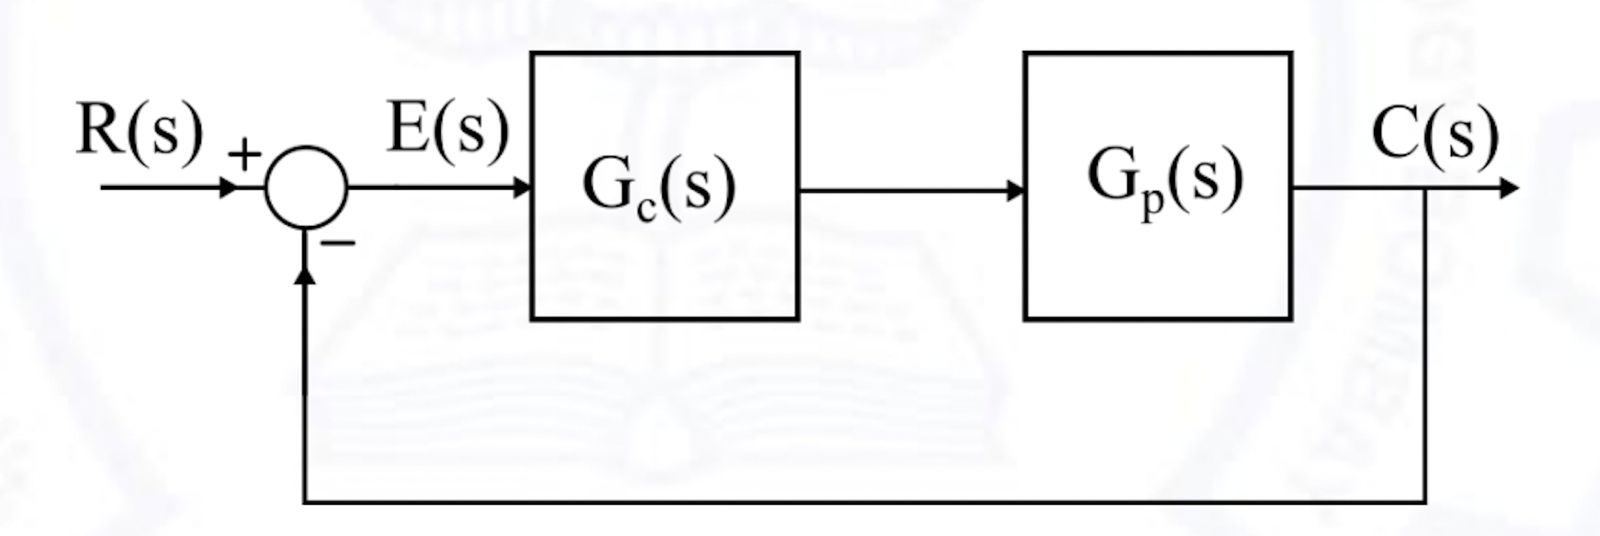
\includegraphics[width=\columnwidth]{2021/EE/46/figs/dia.png}
    \label{fig:ee.46.2021}
\end{figure}
\solution 
 \iffalse
\let\negmedspace\undefined
\let\negthickspace\undefined
\documentclass[journal,12pt,twocolumn]{IEEEtran}
\usepackage{amssymb}
\usepackage{cite}
\usepackage{amsmath,amssymb,amsfonts,amsthm}
\usepackage{algorithmic}
\usepackage{graphicx}
\usepackage{textcomp}
\usepackage{xcolor}
\usepackage{txfonts}
\usepackage{listings}
\usepackage{enumitem}
\usepackage{mathtools}
\usepackage{gensymb}
\usepackage{comment}
\usepackage[breaklinks=true]{hyperref}
\usepackage{tkz-euclide} 
\usepackage{listings}
\usepackage{gvv}                                        
\def\inputGnumericTable{}                                 
\usepackage[latin1]{inputenc}                                
\usepackage{color}                                            
\usepackage{array}                                            
\usepackage{longtable}                                       
\usepackage{calc}                                             
\usepackage{multirow}                                         
\usepackage{hhline}                                           
\usepackage{ifthen}                                           
\usepackage{lscape}
\usepackage{pgfplots}
\newtheorem{theorem}{Theorem}[section]
\newtheorem{problem}{Problem}
\newtheorem{proposition}{Proposition}[section]
\newtheorem{lemma}{Lemma}[section]
\newtheorem{corollary}[theorem]{Corollary}
\newtheorem{example}{Example}[section]
\newtheorem{definition}[problem]{Definition}
\newcommand{\BEQA}{\begin{eqnarray}}
\newcommand{\EEQA}{\end{eqnarray}}
\newcommand{\define}{\stackrel{\triangle}{=}}
\theoremstyle{remark}
\newtheorem{rem}{Remark}
\begin{document}

\bibliographystyle{IEEEtran}
\vspace{3cm}

\title{GATE.2021.EE.46}
\author{EE22BTECH11004 - Allu Lohith}

\maketitle
\newpage
\bigskip

\renewcommand{\thefigure}{\theenumi}
\renewcommand{\thetable}{\theenumi}

Consider a closed-loop system as shown, $$G_p\brak s= \frac{14.4}{s\brak{1+0.1s}}$$ is the plant transfer function and $G_c\brak s=1$ is the compensator. For a unit-step input, the output response has damped oscillations. The damped natural frequency is $\underline{\hspace{2cm}}$
$rad/s$. (Round off to 2 decimal places.)

\begin{figure}[h]
    \centering  
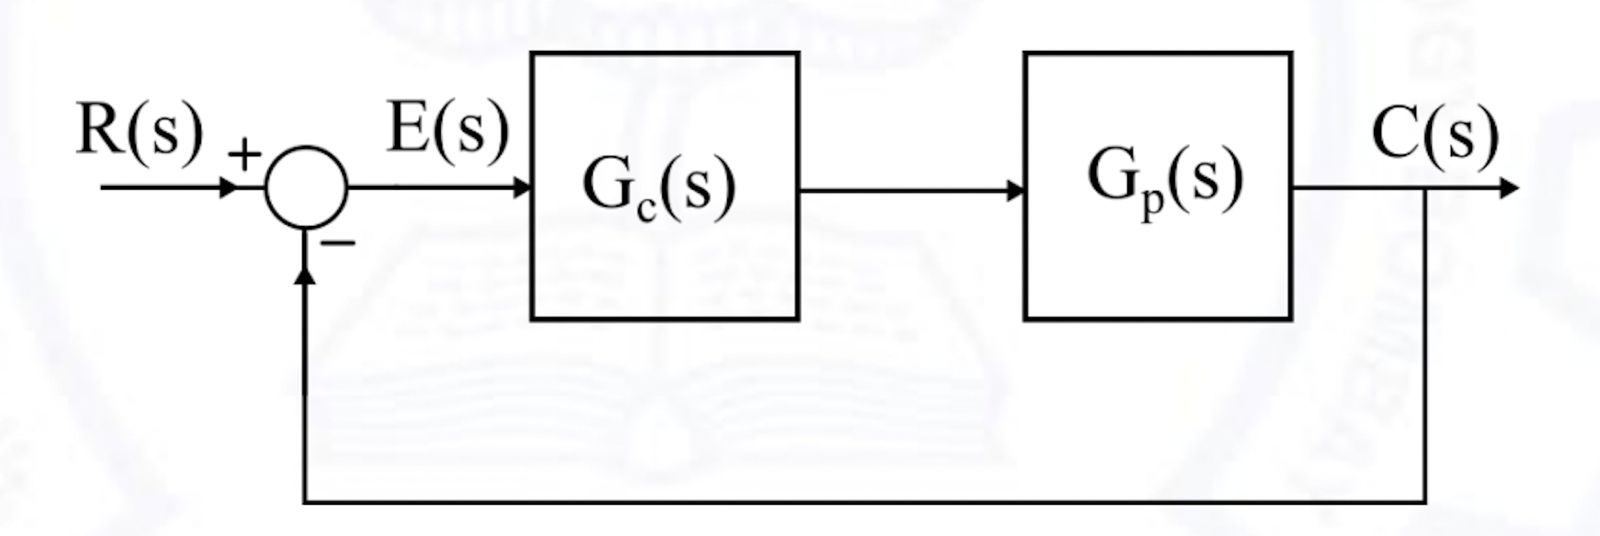
\includegraphics[width=\columnwidth]{2021/EE/46/figs/dia.png}
    \label{fig:ee.46.2021}
\end{figure}
\solution 
\fi
\begin{table}[h!]
\centering
\renewcommand{\arraystretch}{2}
\begin{tabular}{|p{2cm}|p{3cm}|p{2cm}|}
\hline 
\setlength{\tabcolsep}{1pt}
\textbf{Parameter}  &\textbf{Description} &\textbf{Value} \\
\hline
$G_n\brak s$ & Plant transfer function & $\dfrac{14.4}{s\brak{1+0.1s}}$ \\
\hline
$G_c\brak{s}$ &Transfer function of the compensator  & 1 \\
\hline
$\omega_n$ & Damped natural frequency& - \\
\hline
$T$& Overall tranfer function & $\dfrac{C}{R}$\\
\hline
\end{tabular}

\vspace{0.5cm}
\caption{\normalsize Parameters}
\end{table}
As we know that:
\begin{align}
E&=R_c-C_c\\
EG_cG_p&=C
\end{align}
So,
\begin{align}
E &= \frac{Cs\brak{1+0.1s}}{14.4}\\
\frac{Cs\brak{1+0.1s}}{14.4} &=R-C\\
R &=C\brak{\frac{s\brak{1+0.1s}}{14.4}+1}\\
\frac{C}{R} &= \frac{14.4}{0.1s^2+s+14.4}
\end{align}
The characteristic equation is $0.1s^2+s+14.4$ which is of the form $s^2 + 2\zeta\omega_n s + \omega_n^2$, So 
\begin{align}
    \omega_n^2&=144\\
    \omega_n&= 12rad/s
\end{align}

\begin{figure}[h]
    \centering  

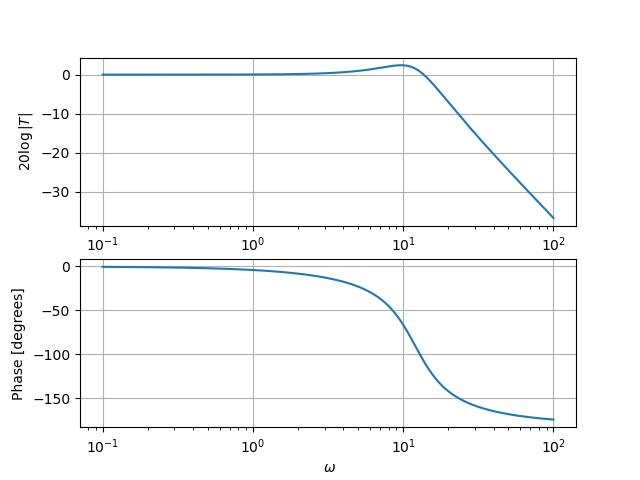
\includegraphics[width=\columnwidth]{2021/EE/46/figs/plot.png}

    \centering
    \caption{Bode Plot - Magnitude and Phase Response}

    \label{fig:ee2.46.2021}
\end{figure}



\pagebreak
\end{enumerate}
